\chapter{Corda Vibrante}

\section{Introduzione}

Obiettivo di questo esperimento è lo studio della propagazione di onde elastiche su una corda fissata ad un estremo, sotto l'azione di una forzante con andamento sinusoidale. Verifichiamo la dipendenza della frequenza dell'onda ($\nu_n$) dalla lunghezza della corda, dalla sua massa lineare ($\mu$) e dalla tensione ($T$) applicata su di essa. Tali grandezze sono infatti legate dalle seguenti relazioni:
\begin{center}
\begin{tabular}{c c c}
$
v= \sqrt{\frac{T}{\mu}} 
$
&
\hspace{1cm}
$
v= \nu_{n} \lambda_n
$ 
&
\hspace{1cm}
$
\lambda_n= \frac{2L}{n} 
$
\\
\end{tabular}
\end{center}

da cui:

\begin{equation}
\nu_n=\frac{n}{2L}\sqrt{\frac{T}{\mu}}
\end{equation}

con $n$ numero intero, al cui variare corrispondono differenti armoniche.


\section{Strumenti}

La strumentazione di cui ci siamo serviti si componeva di due corde:\\

\begin{tabular}{c c c c}
\textbf{Corda A} & \hspace{1cm} $L_A= 2.46\ m$ & \hspace{1cm} $m_A=5.21\cdot10^{-3}\ kg$ & \hspace{1cm} $\mu_A= 2.12\cdot10^{-3}\ kg/m$\\
\textbf{Corda B} & \hspace{1cm} $L_B= 2.50\ m$ & \hspace{1cm} $m_B=1.63\cdot10^{-2}\ kg$ & \hspace{1cm} $\mu_B= 6.52\cdot10^{-3}\ kg/m$\\
\end{tabular} 
\\

La forzante è data da un oscillatore elettromeccanico, mentre la tensione è esercitata da pesetti appesi all'estremità libera della corda, sospesi attraverso una carrucola (come illustrato in \textbf{figura}). 
L'errore associato alla misura di $L_A$ ed $L_B$ è di $\pm0.001\ m$; quello sulle masse è del tutto trascurabile. 

\section{Ricerca delle armoniche}

Nella prima parte dell'esperienza abbiamo verificato che le armoniche superiori sono date da multipli interi della frequenza fondamentale. A tal fine, dopo aver trovato la frequenza di risonanza \textbf{corrispondente ad $n=1$ (ossia la fondamentale)}, facendo variare la frequenza dell'oscillatore elettromeccanico e cercando il punto in cui la corda presentava i nodi alle due estremità e un grande ventre al centro, abbiamo misurato le frequenze relative alle prime cinque armoniche, cui corrispondono le configurazioni descritte in \textbf{figura}. 
\\

Abbiamo ripetuto la misurazione sottoponendo la corda a quattro differenti forze di tensione, e successivamente abbiamo ripetuto l'esperienza per l'altra corda, di massa lineare differente. \\
In tabella sono riportati i valori delle frequenze di risonanza registrate dall'oscillatore elettromeccanico: in verticale si può leggere la dipendenza dalla variazione di tensione per valori crescenti delle masse appese, in orizzontale dal numero di armonica.
\\

\begin{center}
\begin{tabular}{c     c}
\textbf{Corda A} & \textbf{Corda B}\\
\\
\begin{tabular}{ c | c | c | c | c | c }
Massa($g$) & 1 & 2 & 3 & 4 & 5\\
\midrule
550 & 23.7 & 45.5 & 71.3 & 94.6 & 119.6\\
450 & 21,4 & 42,6 & 63,4 & 85,3 & 108,9\\
350 & 19.6 & 37.8 & 57.4 & 76.3 & 95.0\\
250 & 16.1 & 33.1 & 48.7 & 63.4 & 81.3 \\
\end{tabular}
&
\hspace{1cm}

\begin{tabular}{ c | c | c | c | c | c }
Massa($g$) & 1 & 2 & 3 & 4 & 5\\
\midrule
1050 & 19.3 & 38.4 & 56.1 & 75.2 & 94.7 \\
550 & 14.1 & 26.8 & 40.8 & 55.0 & 69.9 \\
450 & 13.1 & 25.4 & 38.9 & 51.7 & 64.2\\
350 & 10.9 & 22.8 & 35.2 & 46.9 & 58.3\\
\end{tabular}

\end{tabular}
\end{center}


Nel seguente grafico mostriamo la relazione tra la frequenza $\nu$ e il numero di armonica $n$. Per rendere più leggibile il grafico ci siamo limitati a rappresentare tale relazione per la corda A sottoposta ad una tensione $T=(0.250\ kg)(9.81\ m/s^2)$. Come ci si aspettava si tratta di una relazione lineare, in accordo con la \textbf{1.1}

%Grafico con i punti.

Abbiamo dunque interpolato i dati con la \textbf{1.1}, utilizzando il metodo dei minimi quadrati, nel caso di una retta passante per l'origine.

\begin{center}
\begin{tabular}{c c}
$m=\frac{\displaystyle\sum{x_i y_i}}{\displaystyle\sum{x_i^2}}$ & \hspace{2cm} $\sigma_m=\frac{\displaystyle\sigma_y}{\sqrt{\displaystyle\sum{x_i^2}}}$
\end{tabular}
\end{center}

Teniamo come variabili indipendenti le $n_i$, le $y_i$ sono ovviamente le frequenze corrispondenti (l'incertezza associata è stata ricavata sperimentalmente e vale $\pm0.5\ Hz$), mentre i parametri da interpolare sono $m=\frac{1}{2l}\sqrt{\frac{T}{\mu}}$ (coefficiente angolare della retta).
$l=1.11\pm0.01\ m$ \footnote{In questo caso l'incertezza sulla lunghezza è stata stimata di un centimetro nonostante quella dello strumento fosse solo di 0.001 m, imputando tale incertezza ad eventuali errori degli sperimentatori: la misurazione infatti richiedeva di prendere come estremo il punto di tangenza con la carrucola, un'operazione in cui era difficile essere veramente accurati.}
è la distanza tra i punti di sospensione della corda: il primo coincide con il punto di applicazione della forzante, il secondo è dato dal punto di tangenza con la carrucola.  

Dall'interpolazione ricaviamo: $m=16.1\pm0.1$ Dunque, moltiplicando $m$ per $2l=2.22\pm0.02\ m$ e propagando l'errore:
$$\sigma_v=\sqrt{\left(\frac{\sigma_m}{m}\right)^2+\left(\frac{\sigma_l}{l}\right)^2}=0.35$$
otteniamo $$v=35.7\pm0.35\ m/s$$ 
Calcoliamo il  $\chi^2$ e otteniamo un valore di $0.8$. La funzione è perfettamente in accordo.  
Confrontiamo il valore trovato con quello ottenuto dall'equazione:
$$v=\sqrt{\frac{T}{\mu}}=\sqrt{\frac{2.45\ N}{2.12 \cdot10^{-3}\ kg/m}}=34.0\ m/s$$

L'errore è:
$$4\% \leq \frac{\delta_v}{v} \leq 5\% $$




\begin{center}

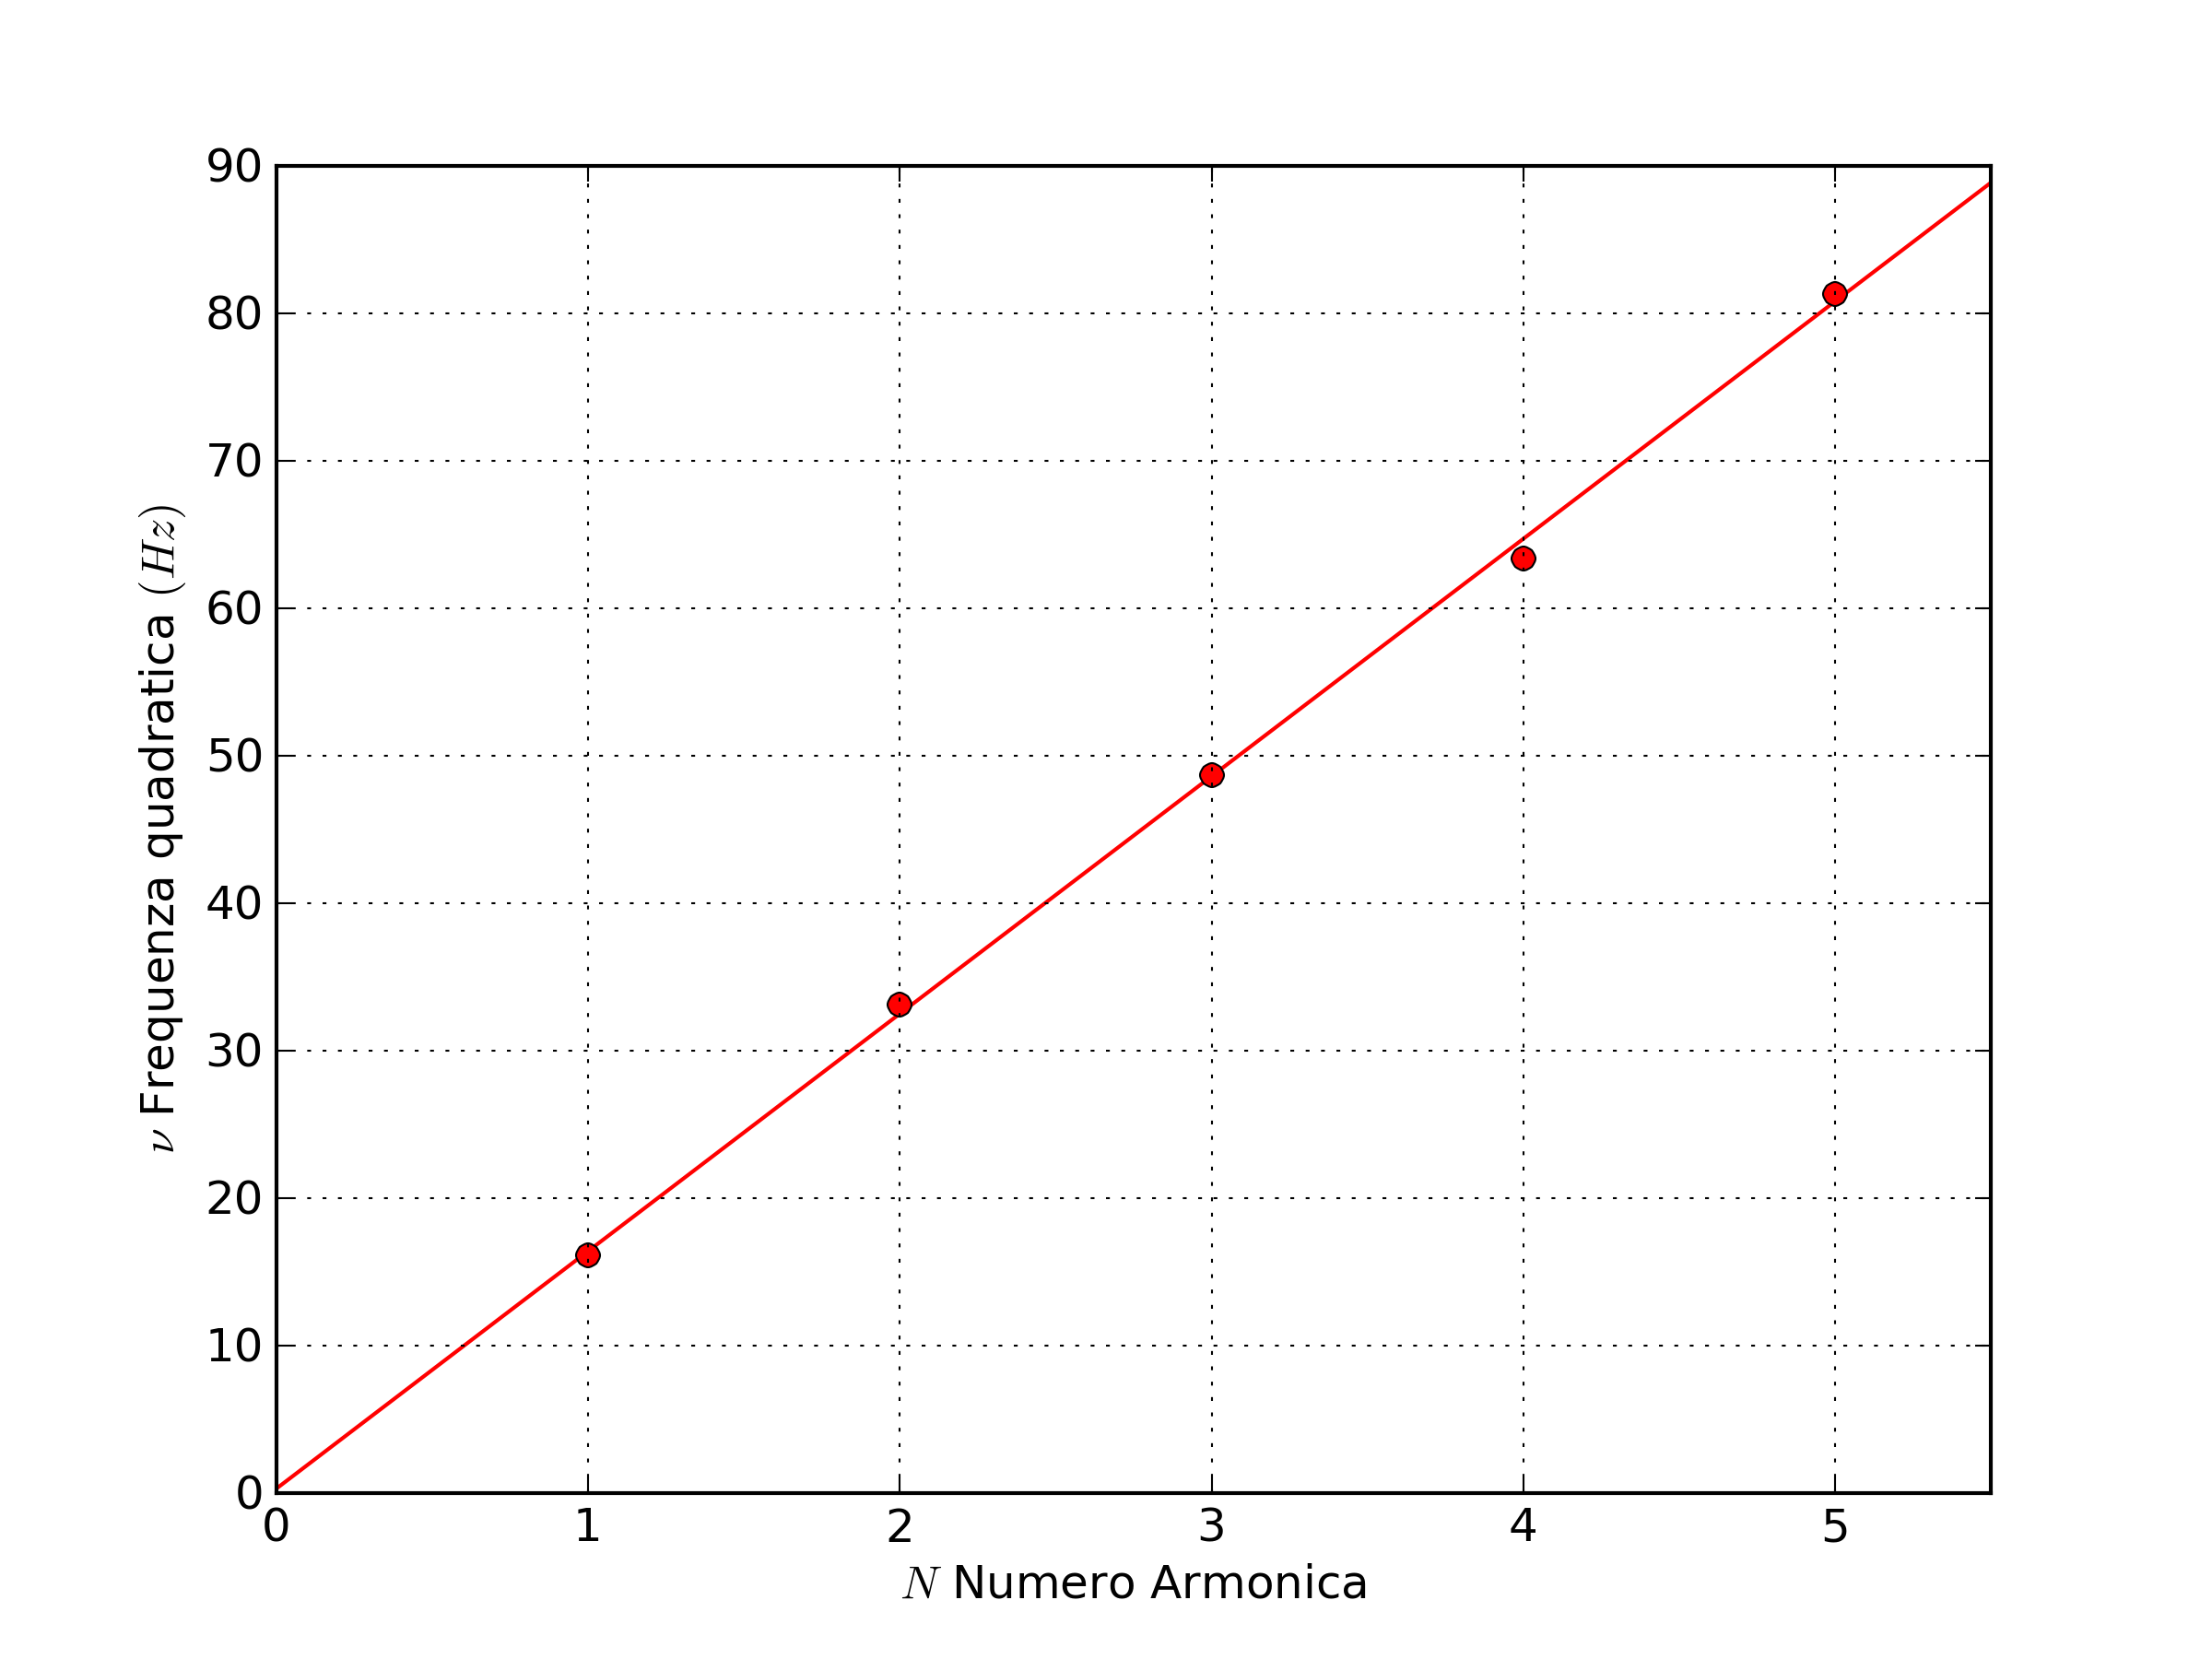
\includegraphics[scale=0.5]{../grafici/corda_1armonica}
\end{center}


\section{Dipendenza dalla tensione}
Dall'equazione $1.1$ si deduce la dipendenza quadratica tra la tensione $T$ e la frequenza $\nu$. 
Verifichiamo questa dipendenza utilizzando i dati della seconda armonica misurati precedentemente. 
\begin{center}
\begin{tabular}{c | c}

\textbf{Corda A}
\begin{tabular}{c|c}
Tensione $N$ & Frequenza $Hz$ \\
\midrule
2.45 & 33.1\\
3.43 & 37.8\\
4.41 &42.6\\
5.39 &45.6\\
\end{tabular}
&\textbf{Corda B}
\begin{tabular}{c|c}
Tensione $N$ & Frequenza $Hz$ \\
\midrule
3.45 & 22.8\\
4.41 & 25.4\\
5.39 & 26.8\\
10.3 & 38.4\\
\end{tabular}
\\
\end{tabular}
\end{center}


 Di seguito il grafico che rappresenta la relazione tra $\nu^2$ e $\tau$.
\begin{center}
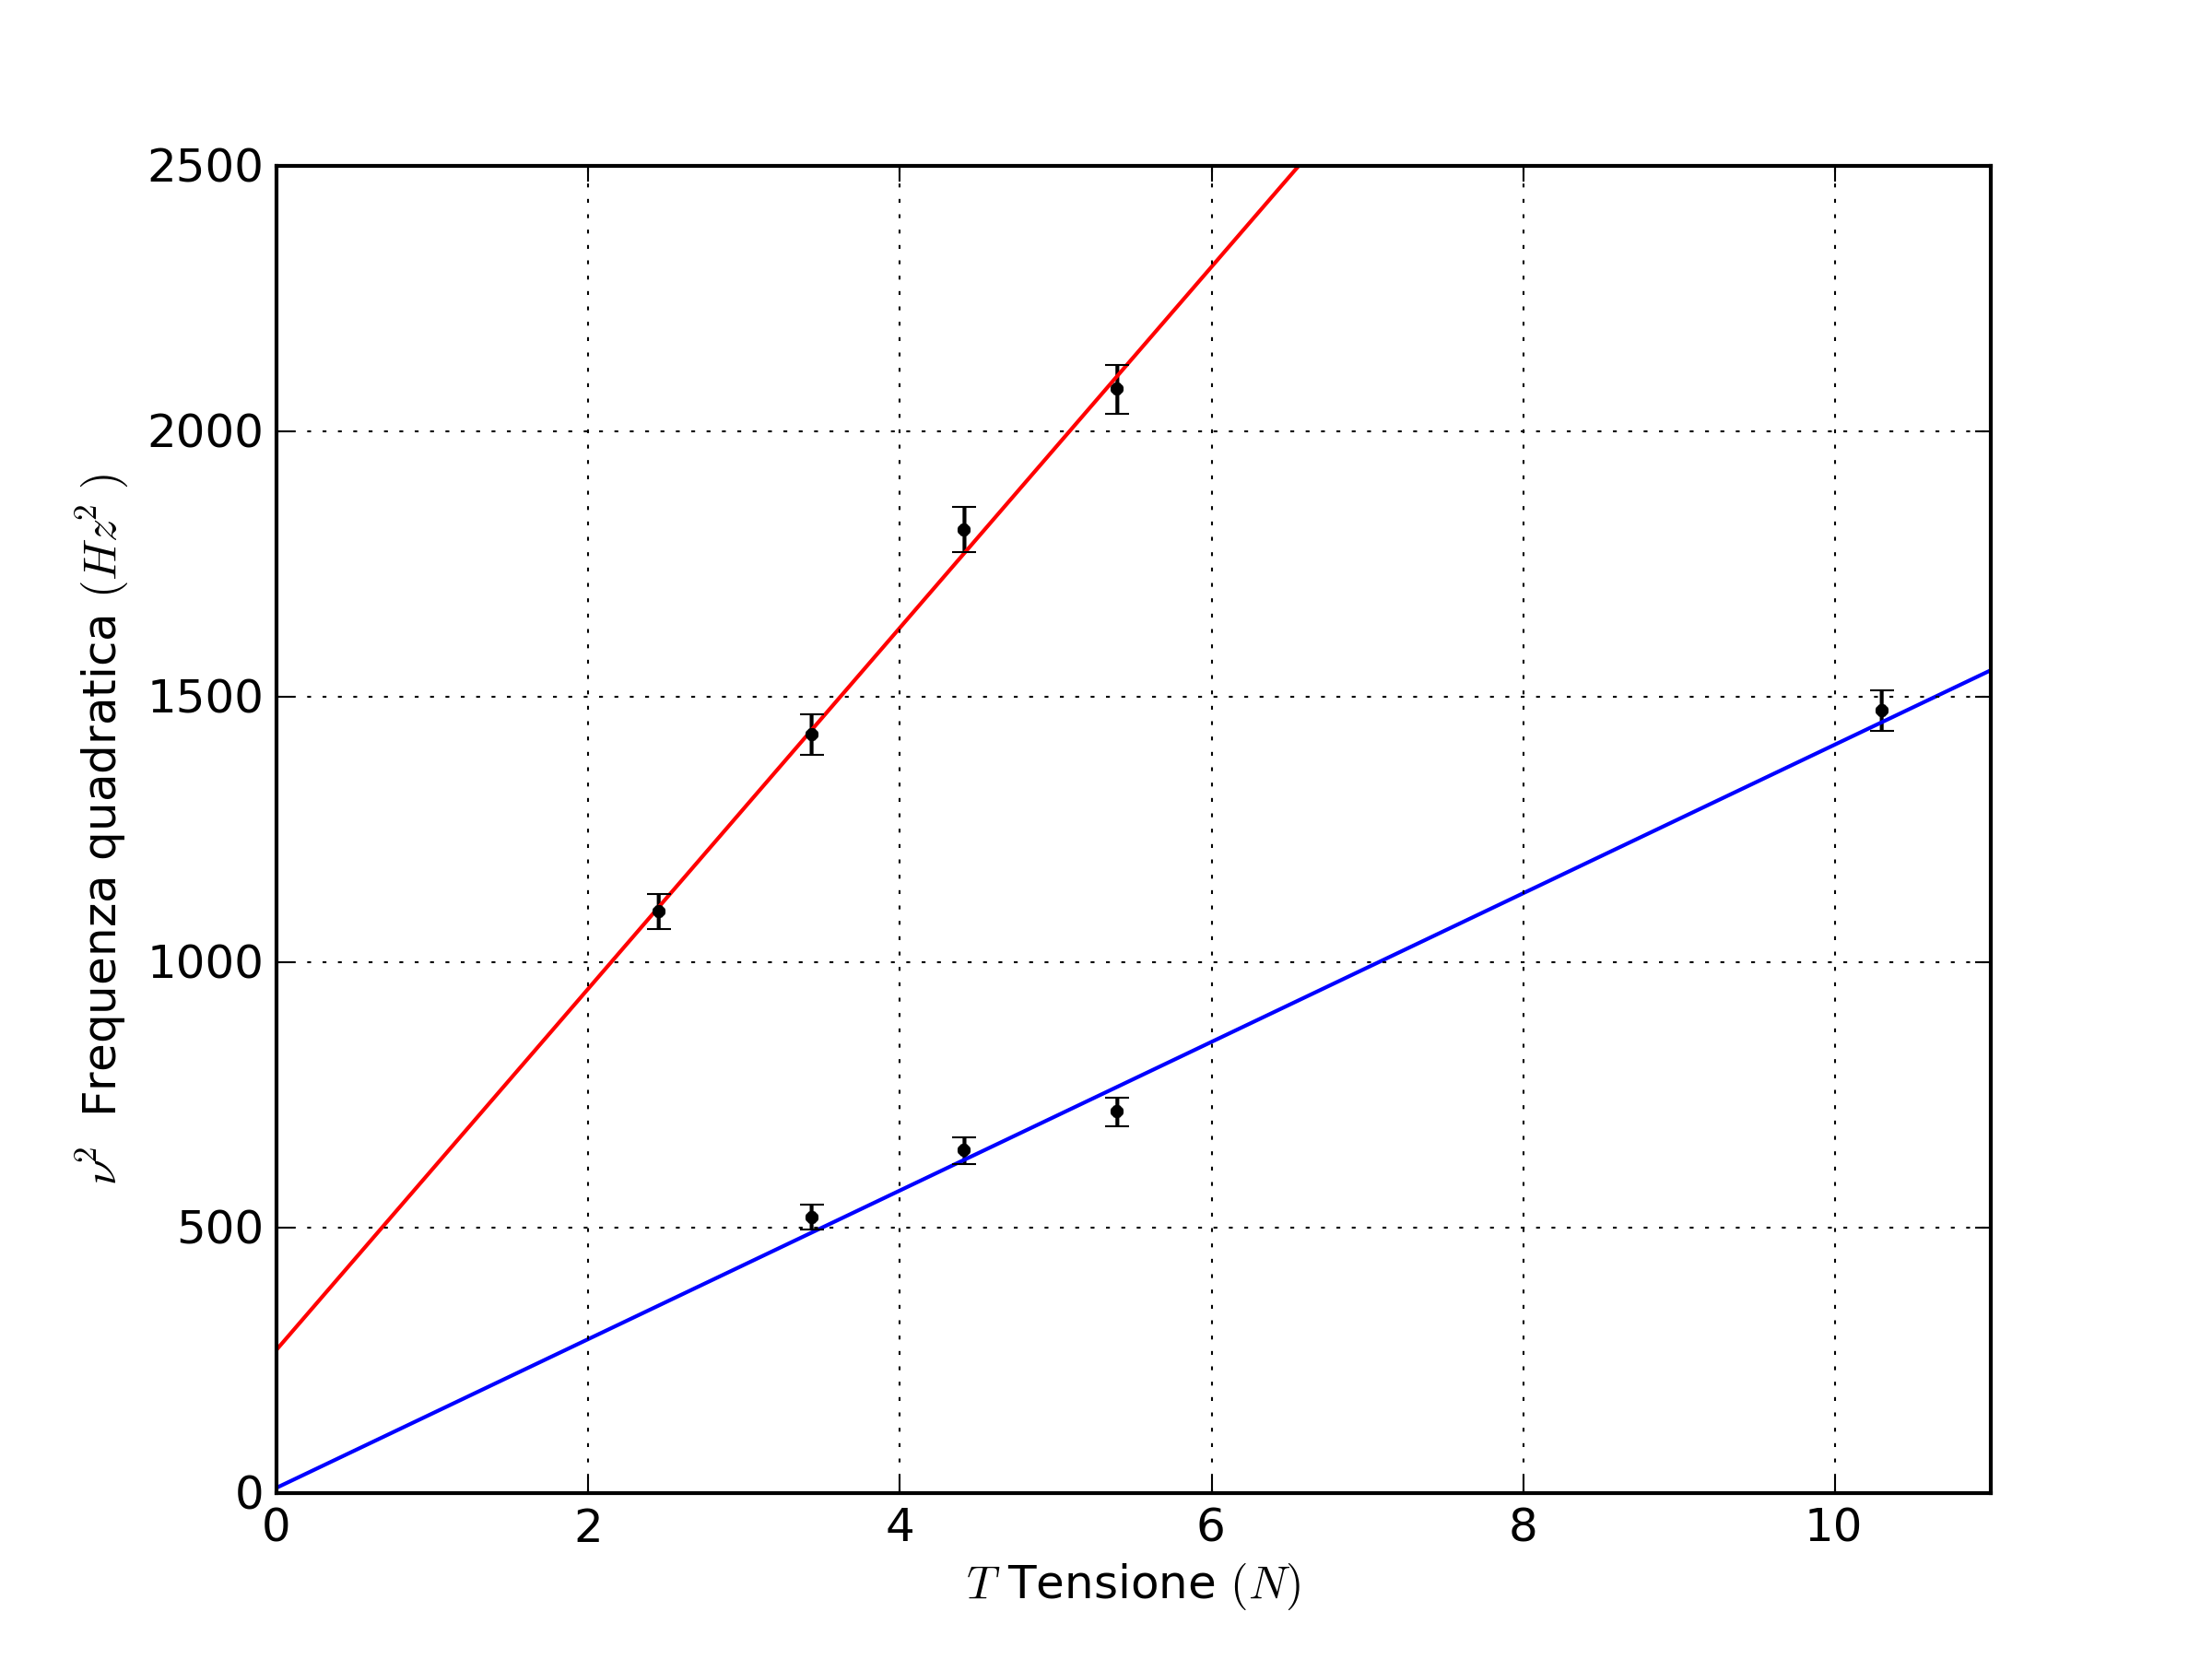
\includegraphics[scale=0.5]{../grafici/corda_tensione}
\end{center}

Si può chiaramente vedere la dipendenza lineare, tra $\nu^2$ e $\tau$. 


\section{Dipendenza dalla lunghezza}
L'ultima analisi riguarda la dipendeza di $\nu_n$ dalla lunghezza della corda, per una data tensione fissata. Essa è ancora una conseguenza della $1.1$, dalla quale si deduce che le due grandezze sono legate da proporzionalità inversa.\\
 
Di seguito sono riportati in tabella i valori raccolti per la prima armonica, per le corde A e B; sono stati scelti valori differenti per le due tensioni in quanto la corda a massa lineare maggiore aveva una risposta poco significativa quando soggetta alla tensione che si era usata per la corda A.\\

\begin{center}


\begin{tabular}{c c}

\textbf{Corda A},  $T=5.40\ N$ & \hspace{3cm} \textbf{Corda B},  $T=10.3\ N$\\
\\
\begin{tabular}{|c|c|}
\toprule
L($m$) & $\nu (Hz) $ \\
\midrule
1.05 & 24.6\\
1.11 & 23.7\\
1.17 & 22.8 \\
1.23 & 20.9 \\
1.32 & 20.1 \\
\bottomrule
\end{tabular}
 
& \hspace{3cm}

\begin{tabular}{|c|c|}
\toprule
L($m$) & $\nu (Hz) $ \\
\midrule
1.10 & 19.33 \\
1.15 & 18.25 \\
1.17 & 17.75 \\
1.22 & 17.00 \\
1.34 & 15.69 \\
1.53 & 13.92 \\
1.60 & 12.96 \\
0.91 & 22.83 \\
0.75 & 27.85 \\
0.60 & 35.00 \\
0.50 & 42.67 \\
\bottomrule
\end{tabular}

\end{tabular}

\end{center}



Il grafico seguente illustra il comportamento della corda B.

\includegraphics[scale=0.75]{"../grafici/CordaPrimaArmonica"}


\section{Conclusioni}
Abbiamo verificato l'equazione 1.1, mostrando la dipendenza della frequenza dalla lunghezza, dalla tensione e dalla massa lineare. 
